\documentclass{article}

\usepackage{RepSty}
\usepackage{SPINDefs}
\usepackage{hyperref}

\usepackage{setspace}
\usepackage{multirow}
\usepackage{threeparttable}
\usepackage{paralist}

\usepackage[caption=false]{subfig}

\begin{document}
	
	\singlespacing
	\begin{titlepage}

\begin{center}
{МИНИСТЕРСТВО ОБРАЗОВАНИЯ И НАУКИ РОССИЙСКОЙ ФЕДЕРАЦИИ}\\[3pt]
\textsc{\small{Федеральное государственное автономное образовательное учреждение высшего образования}}\\

\textbf{\enquote{Национальный исследовательский ядерный университет\\
{``МИФИ''}}}\\
\textbf{(НИЯУ МИФИ)}\\[2cm]




\textsc{\textbf{Практическое задание по курсу ``Научная визуализация''}}\\[2cm]

% Title
\enquote{Визуализация данных сечения взаимодействия поляризованных пучка и мишени в эксперименте по изучению временной инвариантности TRIC.}\\[2cm]


\end{center}


\begin{flushleft}
% Author and supervisor
\begin{tabular}{ll}
	Аспирант                   & А.Е. Аксентьев                           \\
	Направление                & 03.06.01 Физика и астрономия             \\
	Научная специальность      & 01.04.20 Физика пучков заряженных частиц \\
	                           & \-\hspace{1.8cm} и ускорительная техника \\[1cm]
	Преподаватель       &                                          \\
	ФИО, степень, звание & В.В. Пилюгин, к.т.н, доц.             \\[1cm]
	Дата защиты:               &                                          \\
	Результат защиты:          &
\end{tabular}

\end{flushleft}

\vfill


\begin{center}
Москва \the\year{}
\end{center}



\end{titlepage}
	
	\tableofcontents 
%	\pagebreak
	
	\onehalfspacing
	
	\section{Задание исходных данных}
	
	В работе изучалось полное сечение взаимодействия поляризованного протонного пучка и поляризованной дейтериевой мишени. В качестве исходных данных использовались измерения полного тока пучка, представленные на рисунке~\ref{fig:Cycles}, которые затем статистически обрабатывались (путём линейной регрессии логарифма тока) для получения оценки сечения взаимодействия,~\ref{fig:Slopes}. 
	
	Принимая за модель спада тока пучка выражение 
	\[
	I_t  = I_0 \cdot e^{-\nu\CS[0]\Thick \cdot t} \equiv I_0\cdot e^{\slp\cdot t},
	\]
	где $\nu$ --- частота оборота пучка в ускорителе, $\Thick$ --- толщина мишени, $\CS[0]$ --- искомое сечение взаимодействия, $\CS[0]$ можно оценить профитировав логарифм тока, принимая оценку угла наклона прямой $\slp* = -\nu\Thick\cdot \CS*[0]$. ($\nu$ --- известная величина, задаваемая энергией пучка, $\Thick$ оценивается отдельно.)
	
	\begin{figure}[h!]
		\centering
		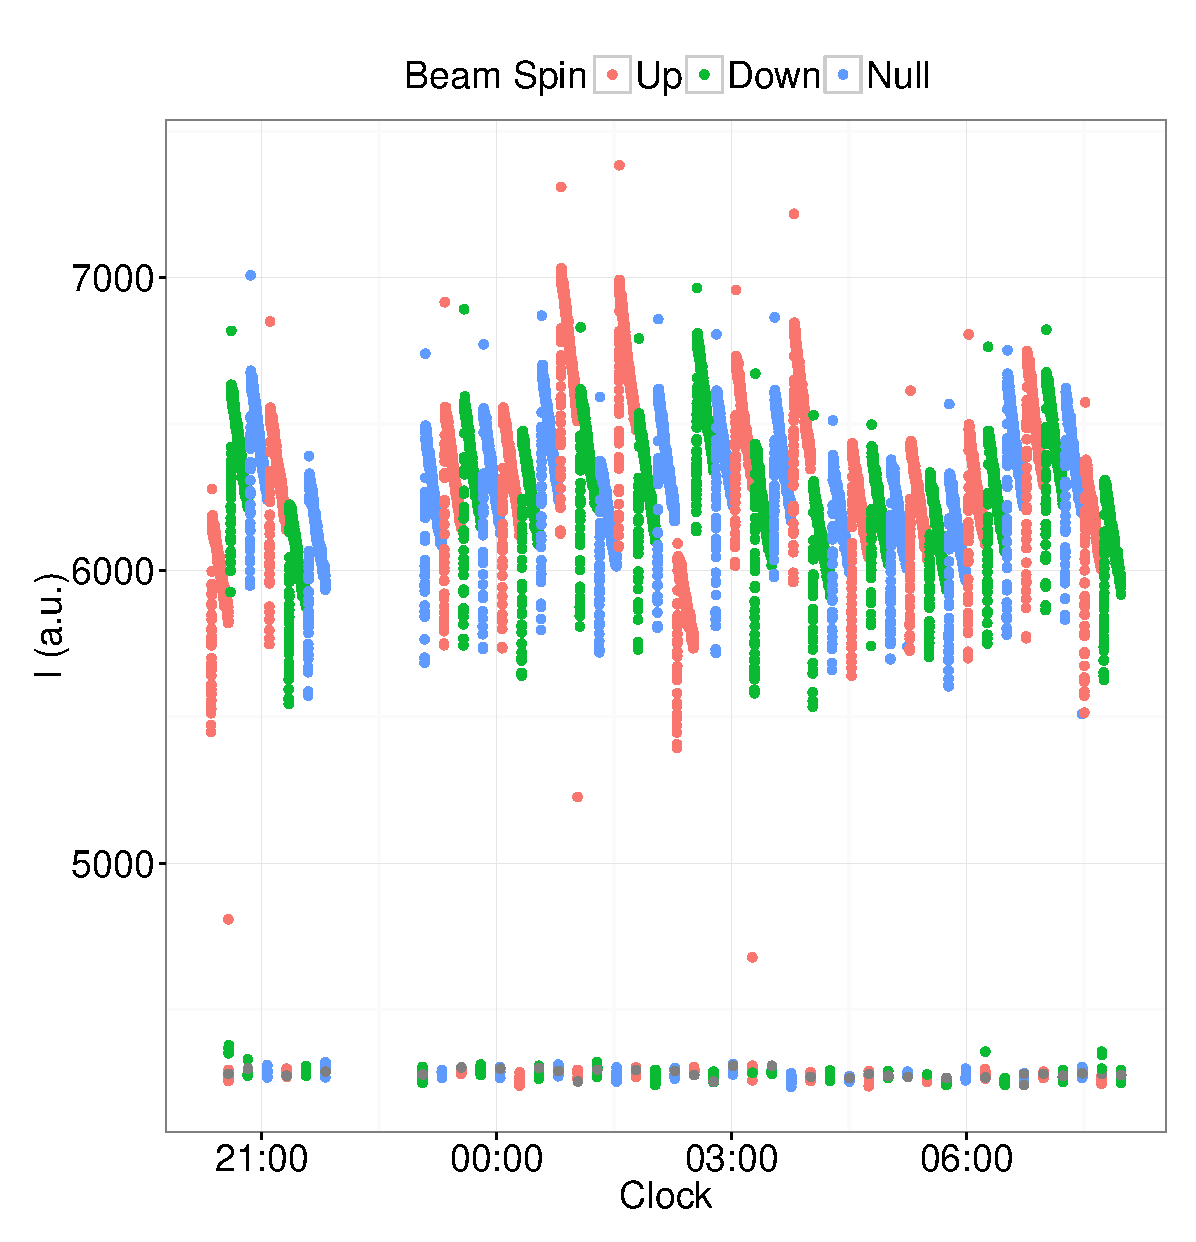
\includegraphics[scale=.7]{Cycles2016.eps}
		\caption{Циклы окрашены в соответствии с состоянием поляризации пучка. До 22:30 спин мишени находится в состоянии 3, после --- в состоянии 1.\label{fig:Cycles}}
	\end{figure}
	\begin{figure}[h!]
		\centering
		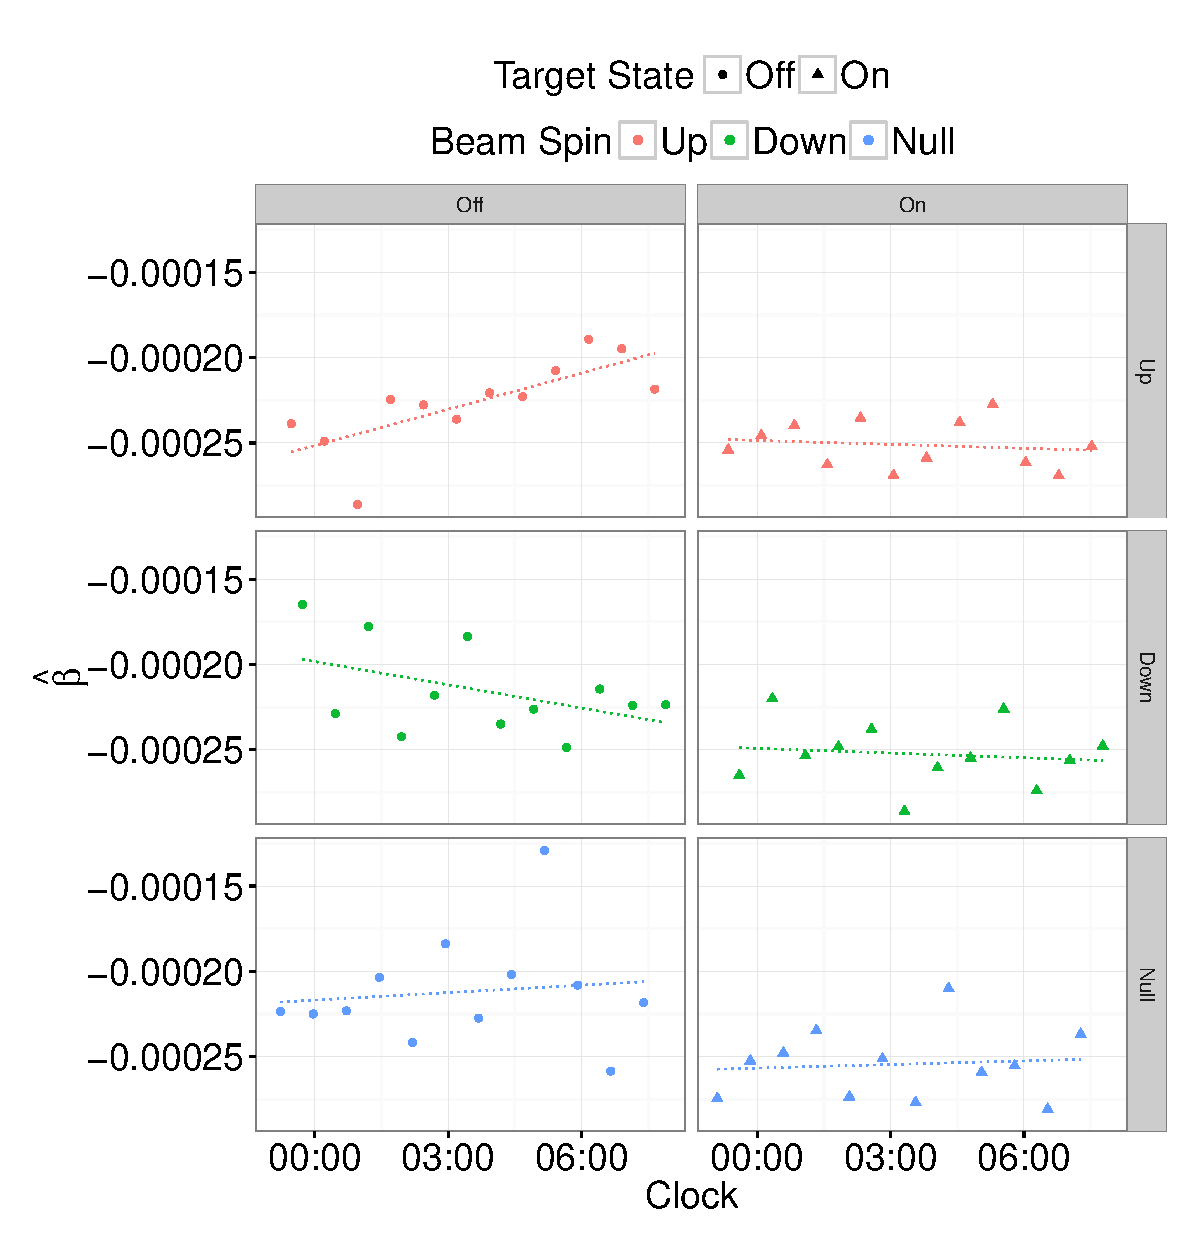
\includegraphics[scale=.7]{Slopes2016_VS_Clock.eps}
		\caption{Оценки сечения взаимодействия при спиновом состоянии мишени 1.\label{fig:Slopes}}
	\end{figure}	
	
	\section{Фильтрация}
	Полученные значения $\slp*$ подвергались тесту диапазона Туки~\cite{Tukey_range_test}; оценки сечения, основанные на аномальных по тесту Туки $\slp*$, были отнесены к категории \emph{Unsound}. Также, оценки классифицировались по критерию близости друг к другу $\slp*$, на основании которых они вычислялись (данная классификация отражает озабоченность нестабильностью условий в ускорителе). Оценки сечений взаимодействия по всем классификационным группам сведены в таблице~\ref{tbl:CS0SumStat}. Оценки из категории \emph{Unsound} не участвуют в конечном представлении данных.
	
	\begin{center}
		\begin{threeparttable}[H]
			\centering
			\caption{Некоторые статистики данных по сечению взаимодействия.\label{tbl:CS0SumStat}}
			\begin{tabular}{llrrrrrr}
				\hline\hline
				Sound                & Close &  \# & Mean\tnote{a} (a.u.) & SE\tnote{b} (a.u.) & $\chi^2_{red}$ & SE\tnote{c} (a.u.) &  Mode\tnote{d} (a.u.)\\ \hline
				\multirow{3}{*}{Yes} & Yes   &  21 &                  366 &                 73 &            6.5 &                178 &  386 \\
				& No    & 111 &                  397 &                 30 &            7.0 &                 80 &  403 \\
				& All   & 132 &                  393 &                 28 &            6.9 &                 73 &  400 \\ \hline
				\multirow{3}{*}{No}  & Yes   &   2 &                 1469 &                 22 &            0.1 &                  5 & 1467 \\
				& No    &  10 &                 1440 &                 83 &            4.2 &                169 & 1429 \\
				& All   &  12 &                 1444 &                 69 &            3.4 &                127 & 1435 \\ \hline
			\end{tabular}
			\begin{tablenotes}
				\item[a]{Средне-взвешенное.}
				\item[b]{Стандартно отклонение делёное на корень из размера выборки.}
				\item[c]{С коррекцией по дисперсии через $\chi^2_{red}$.}
				\item[d]{Наиболее часто встречающееся значение.}
			\end{tablenotes}
		\end{threeparttable}
	\end{center}
	
	\section{Мэппинг и Рендеринг}
	Для визуализации данных используются 2-D графики оценки плотности распределения сечения. Плотность распределения представлена окрашенной гладкой линией, функция $y = f(x)$ которой вычисляется некоторым статистическим алгоритмом~\cite{Density_estimation}. Цвета линий определяются принадлежностью данных категориям \emph{Close}/\emph{Far}.
	
	Рисунок графика плотности распределения сечения взаимодействия был выполнен с использованием визуалиционного пакета GGPlot2~\cite{GGPlot2} (имплементации Хэдли  Уикэмом \emph{Grammar of Graphics} Лиленда Уилкинсона) для статистического языка программирования R.~\cite{GGPLOT2_WIKI} Результат представлен на рисунке~\ref{fig:CS0au_dens}.
	
	\begin{figure}[h!]
		\centering
		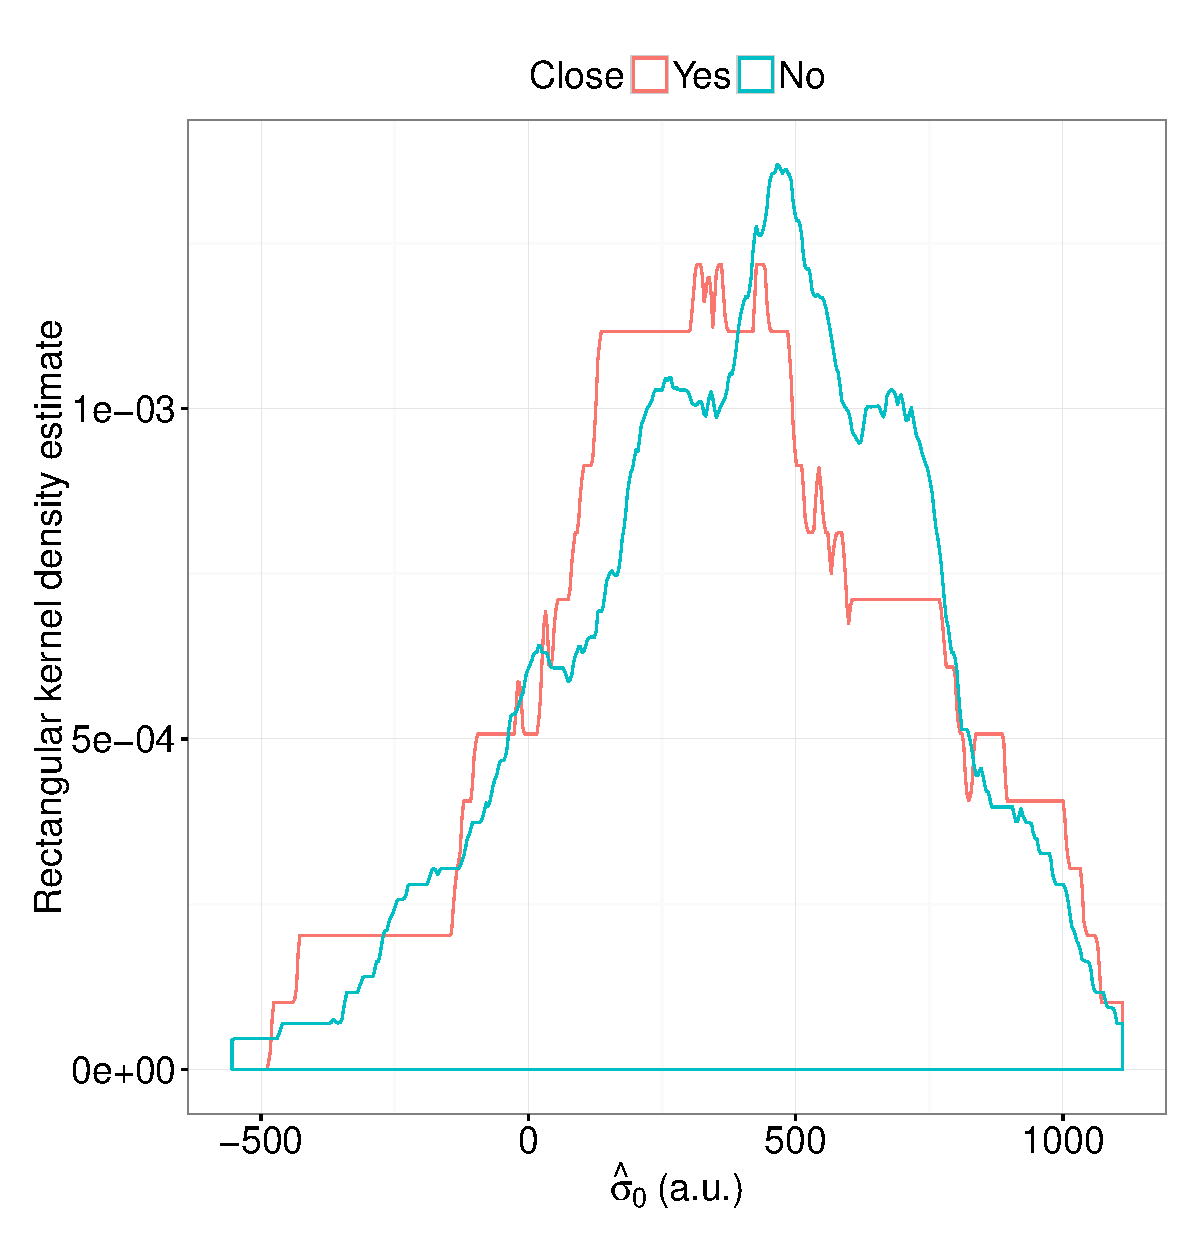
\includegraphics[scale=.7]{CS0_au_dens.eps}
		\caption{Оценка плотности распределения сечения взаимодействия.\label{fig:CS0au_dens}}
	\end{figure}

	\section{Выводы}
	В процессе анализа и визуализации данных были обнаружены возможные систематические эффекты, влияющие на конечный результат; конкретнее, вероятность того, что изменение режима работы вакуумной системы во время эксперимента имеет достаточное влияние на данные по току пучка, что линейная регрессия не является применимым средством анализа (см рис.~\ref{fig:res_vs_fit}).
	
	Также, была обнаружена значительная автокорреляция (на уровне 60\%) отклонений предсказанных моделью значений логарифма тока от измеренных данных (см. рис.~\ref{fig:DW2}), что может свидетельствовать об обратной связи между током пучка и трансформатором тока, которым измеряется этот ток. 
	
	\begin{figure}[h!]
		\centering
		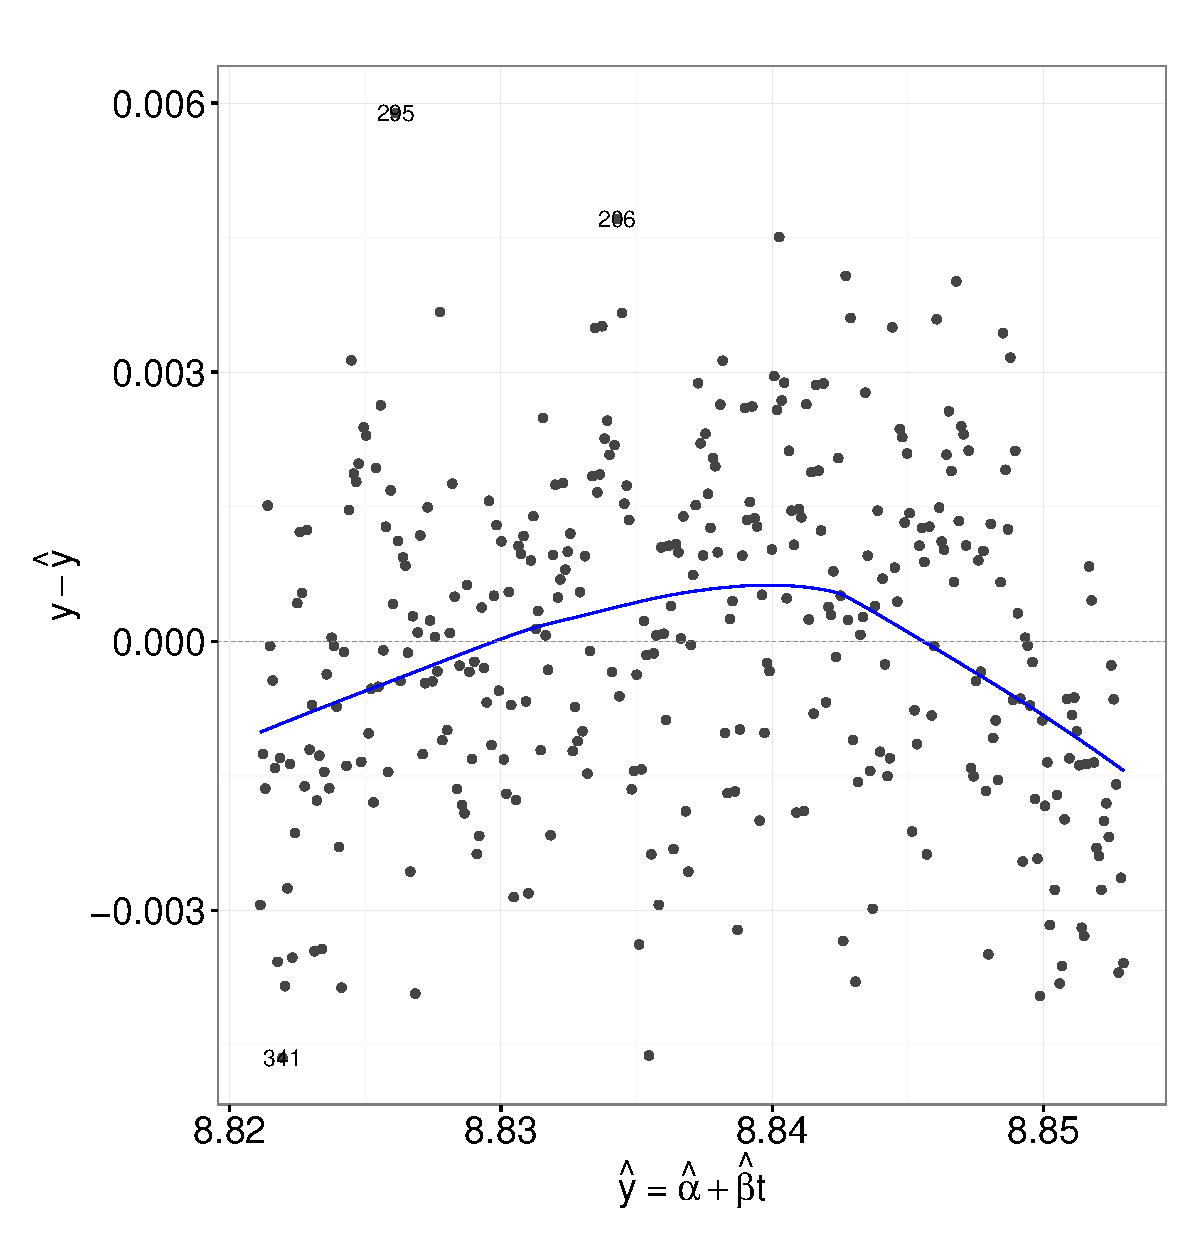
\includegraphics[scale=.7]{Res_VS_Fit_2016-17.eps}
		\caption{График отклонений линейной модели в зависимости от предсказанных моделью значений логарифма тока. U-образная форма говорит о несоответствии линейной модели логарифма тока данным. \label{fig:res_vs_fit}}
	\end{figure}

	\begin{figure}[h!]
		\centering
		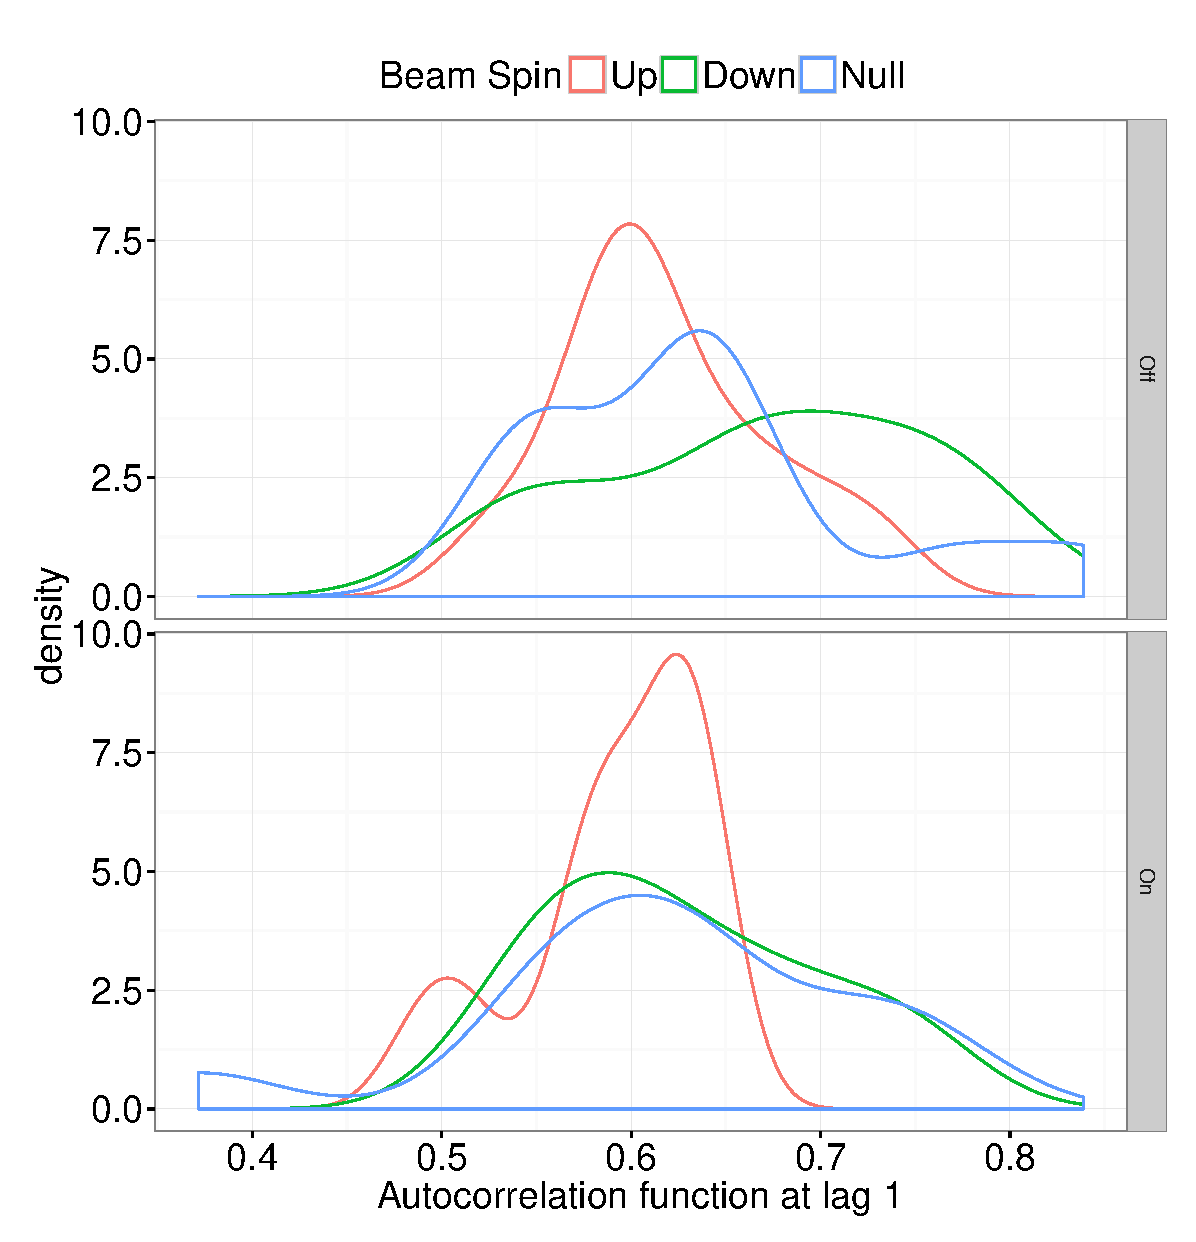
\includegraphics[scale=.7]{ACF1_dens.eps}
		\caption{Распределение автокорреляционной функции отклонений модели на шаге 1. В примерно 60\% данных наблюдается корреляция между соседними измерениями тока пучка.\label{fig:DW2}}
	\end{figure}

	\begin{thebibliography}{9}
		\bibitem{Tukey_range_test}
		Описание теста Туки. \url{https://www.itl.nist.gov/div898/handbook/prc/section4/prc471.htm}
		
		\bibitem{Density_estimation}
		Эмпирическая оценка плотности распределения данных. \url{http://users.stat.umn.edu/~helwig/notes/den-Notes.pdf}
		
		\bibitem{GGPlot2}
		GGPlot2 на CRAN. \url{https://cran.r-project.org/web/packages/ggplot2/index.html}
		
		\bibitem{GGPLOT2_WIKI}
		GGPlot2 статья на википедии. \url{https://en.wikipedia.org/wiki/Ggplot2}
	\end{thebibliography}
	
\end{document}